\documentclass[
    type=projectproposal,
    twocolumn
]{bfhpub}

% Include Packages
\usepackage[main=english]{babel}
 
\begin{document}

\title{Improving the graphical user interface of Vula}
\subject{Making secure communication more accessible by improving the user experience.}
\department{BFH TI}
\titlefooterright{Project Proposal BTI2029}
\advisor{Dr. J. Appelbaum}
\expert{Dr. J. Appelbaum}
\projectpartner{Vula}
\author{Khan Mursel Ijaz, Dedding Sander}


\begin{ProjectDescription}
    \section{Project Description}
    Students that are enrolled in the course BTI2018-25 have the opportunity to make a contribution to a free software project. They will be contributing to Vula. A Tool that provides its users with a way to securely communicate within a local area network. We have chosen to improve the existing graphical user interface (gui). The current version was built with tkinter by students of BFH in a previous iteration of this course. The goal is not to redo the gui but to expand upon it. Vula can be found via Vula.link or Codeberg.org/vula.
\end{ProjectDescription}

\maketitle

\section{Projektziele}
\begin{itemize}
    \item Evaluate the current gui
    \item Itemize and prioritize the areas that need improvement
    \item Come up with solutions to the issues we decide to address
    \item Implement and document the changes
\end{itemize}

\par\nointerlineskip\bfhRule

\textbf{Some issues that we have already identified:}
\begin{itemize}
    \item Example 1: Removing a pinned peer crashes the gui. This should be fixed
    \item Example 2: The Scrollbars should be changed to fit the overall design
    \item Example 3: Currently the gui consists of multiple small windows. Making it into 1 single window would be more organized
    \item Example 4: The process of scanning a verification key is rather clunky and can definitely be streamlined
\end{itemize}

\par\nointerlineskip\bfhRule
 
\newpage

\textbf{What the gui currently looks like:}
\begin{figure}[ht]
    \centering
    \begin{minipage}{0.49\linewidth}
        \centering
        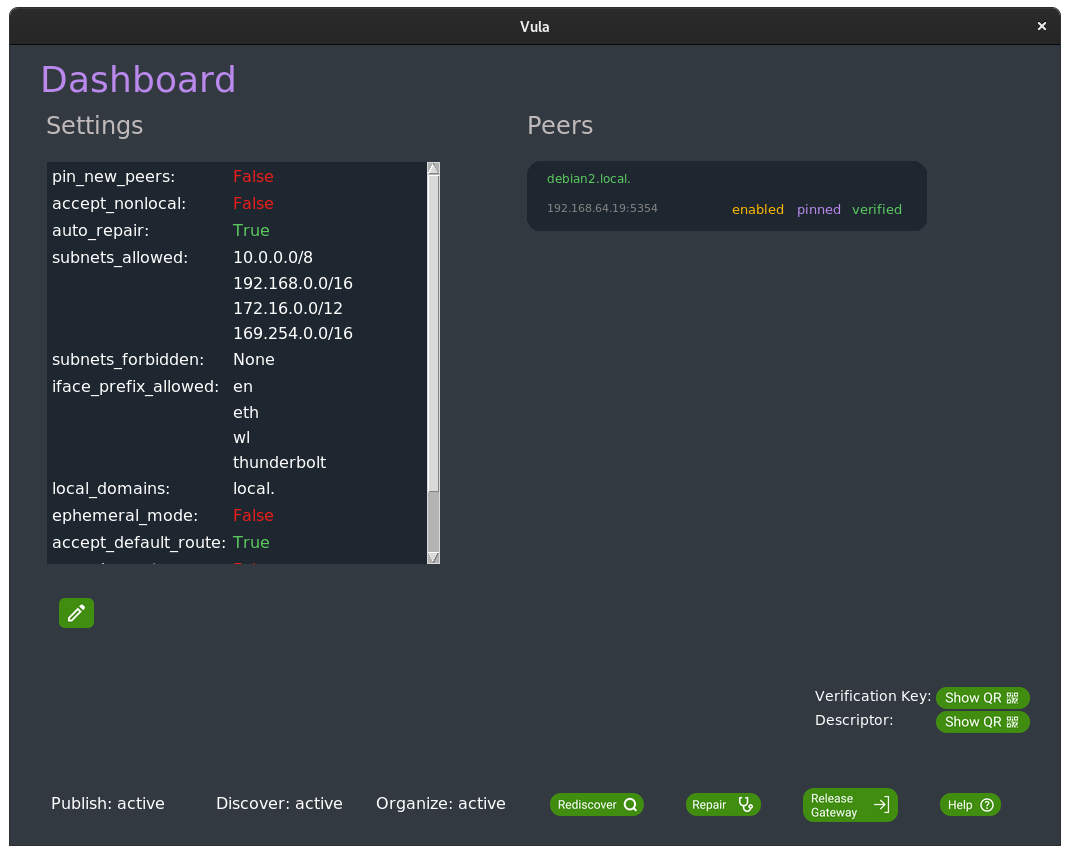
\includegraphics[width=\linewidth]{./../misc/frontend/dashboard.png}
    \end{minipage}\hfill
    \begin{minipage}{0.49\linewidth}
        \centering
        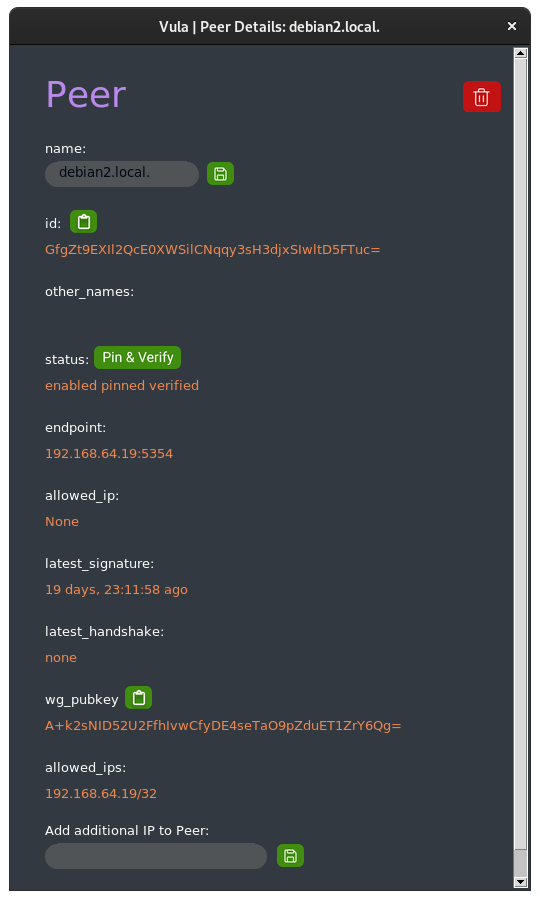
\includegraphics[width=\linewidth]{./../misc/frontend/peer.png}
    \end{minipage}
    \caption{Current GUI Screenshots}
\end{figure}

\par\nointerlineskip\bfhRule

\end{document}